\documentclass[a4paper]{article}

%% Language and font encodings
\usepackage[english]{babel}
\usepackage[utf8x]{inputenc}
\usepackage[T1]{fontenc}
\usepackage{listings}

%% Sets page size and margins
\usepackage[a4paper,top=3cm,bottom=2cm,left=3cm,right=3cm,marginparwidth=1.75cm]{geometry}

%% Useful packages
\usepackage{amsmath}
\usepackage[colorinlistoftodos]{todonotes}
\usepackage[colorlinks=true, allcolors=blue]{hyperref}
\usepackage{listings}
\usepackage{url}
\usepackage{graphicx}
\graphicspath{ {./images/} }
% \DeclareGraphicsExtensions{.pdf,.jpg,.png}

%% defined colors
\definecolor{Blue}{rgb}{0,0,0.5}
\definecolor{Green}{rgb}{0,0.75,0.0}
\definecolor{LightGray}{rgb}{0.6,0.6,0.6}
\definecolor{DarkGray}{rgb}{0.3,0.3,0.3}

% \newcommand*\lstinputpath[1]{\lstset{inputpath=#1}}
% \lstinputpath{code/}

\lstset{language=R,
	basicstyle=\ttfamily\small,
	breaklines=true,
	keywordstyle=\bfseries\color{Blue},
	commentstyle=\itshape\color{LightGray},
	stringstyle=\color{Green},
	numbers=left,
	numberstyle=\tiny\color{DarkGray},
	stepnumber=1,
	numbersep=10pt,
	backgroundcolor=\color{white},
	tabsize=2,
	showspaces=false,
	showstringspaces=false,
	captionpos=b,
	%    inputpath={code/},
	frame=tb
}

\lstset{language=Python,
	basicstyle=\ttfamily\small,
	breaklines=true,
	keywordstyle=\bfseries\color{Blue},
	commentstyle=\itshape\color{LightGray},
	stringstyle=\color{Green},
	numbers=left,
	numberstyle=\tiny\color{DarkGray},
	stepnumber=1,
	numbersep=10pt,
	backgroundcolor=\color{white},
	tabsize=2,
	showspaces=false,
	showstringspaces=false,
	captionpos=b,
	%    inputpath={code/},
	frame=tb
}

\title{Assignment 4: Association Rules}
\author{
	Low, Daniel Mark (S3120155) \\
	Petre, Bogdan (S3480941) \\
	Xu, Teng Andrea (S3548120) \\ 
	\\ \textbf{Group} 7}
\date{\today}


\begin{document}
	\maketitle
	
	\section{Introduction: Confidence and Support (30p)}
	
	\textit{1. Question:} What’s the importance of lift in association rule mining? Why is confidence and/or
	support not sufficient?\\
	\textit{1. Answer:} The function of lift is to measure how many times more often the items X and Y occur together than expected if they are are statistically independent of each other. It is a measure of how the two items are really related rather then coincidentally happening together.\\
	The following is the lift formula:
	
	\begin{center}
		$Lift(X\rightarrow Y)=  \frac{Support(X \cap  Y)}{Support(X)*Support(Y)}$ 
	\end{center}
	If the result is equal to 1, then X and Y will seem to be statistically independent of each other. On the other hand, the greater the result is, the stronger the association between the two items.
	
	Confidence is not sufficient because it only takes into account the support of X and not the support of Y. If Y is just as popular as X then there will be a higher probability that a transaction containing X will also contain Y thus increasing the confidence. Lift weighs how popular Y is: if Y is very unpopular, then it will tend to make the overall answer be larger. If the answer is larger than 1, it suggests the itemset Y tends to happen in the presence of itemset X. Less than 1 indicates the itemset Y is unlikely to happen if itemset X happens. So it shows how interesting or relevant the association rule is. \\
	\newline
	\textit{2. Question:} suppose you want to apply association rule mining on a collection of surveys containing
	personal details such as: name, age, gender, hobbies, favorite color, income, country etc.
	How would you convert this raw data into a form suitable for association analysis? \\
	\textit{2.Answer:} First of all the table name gives us nothing, for example if we have lift (name)\{Marco\} $\rightarrow$ (hobby)\{Basketball\} equal to 2 it does not mean anything, it's just coincidence that in the dataset many transaction have Marco that play basketball but statistically it does mean nothing.\\
	Then I will change the continuous data like "age" and "income" in an interval or categorical, for example for age "youth" if the age is below 30 and the wealthy if income(annual) is like 100.000 euros. Then we will have for example lift like (country,job)\{USA,engineer\} $\rightarrow$ \{wealthy\} equal to 2.5, that does make sense.\\  
	\newline
	\textit{3. Question:} Suppose we already know that the lift of the rule wine => cheese is 2. We also know the
	that the support of wine is 0.1. What can we say about the support for cheese?\\
	\textit{3.Answer:} Support(cheese) has to be 5 times Support(wine $\cap$ cheese) because from the previous lift formula we obtain:
	
	\begin{center}
		$Support(cheese) = \frac{Support(wine\cap cheese)}{Support(wine) * Lift(wine \rightarrow cheese)}$
	\end{center}
	So if Support(wine $\cap$ cheese) is 0.1, Support(cheese) is 0.5; So if Support(wine $\cap$ cheese) is 0.05, Support(cheese) is 0.25. That also makes sense because if we have 10\% of all transaction contain wine then the value of Support(wine $\cap$ cheese) has to be lower or equal to Support(wine) (case limit when in all occurrences of wine we have also cheese).\\
	\newline
	\textit{4. Question:} Find all rules with a minimum support of 0.3 and a minimum confidence of 0.7. Give a
	short explanation on how you found these rules.\\
	\textit{4.Answer:} We used \textbf{R} and the package \textbf{arules} to find the rules (see \textit{script\_1\_4.R}). We declared a data frame to with the columns "TID" and "item" and the same rows, then we got a transaction object from it, then we applied the \textbf{apriori} function with the required \textit{support} and \textit{confidence} parameters.
	
	\begin{lstlisting}
	rules   support confidence  lift count
	1   {6} => {5} 0.3333333       1.00 1.500     2
	2   {4} => {3} 0.5000000       1.00 1.500     3
	3   {3} => {4} 0.5000000       0.75 1.500     3
	4   {5} => {3} 0.5000000       0.75 1.125     3
	5   {3} => {5} 0.5000000       0.75 1.125     3
	6 {2,4} => {3} 0.3333333       1.00 1.500     2
	7 {2,3} => {4} 0.3333333       1.00 2.000     2
	8 {4,5} => {3} 0.3333333       1.00 1.500     2
	
	\end{lstlisting}
	
	
	\section{Beethoven and Iron Maiden (70p)}
	\subsection{Loading, cleaning, and plotting data}
	\label{sec:21}
	
	The tsv file is quite large (2.53 GB) so after loading the file, we created a trimmed data frame of only the columns "userid" and "artname", the two variables we will use for the analysis. The raw dataframe had missing values, but none on these two columns (checked with, so no further preprocessing was done. Plots were done in Python (see script\_21.py). To start visualizing the data set, we plot the highest frequency bands of all users:
	\begin{figure}[ht!]
		\centering
		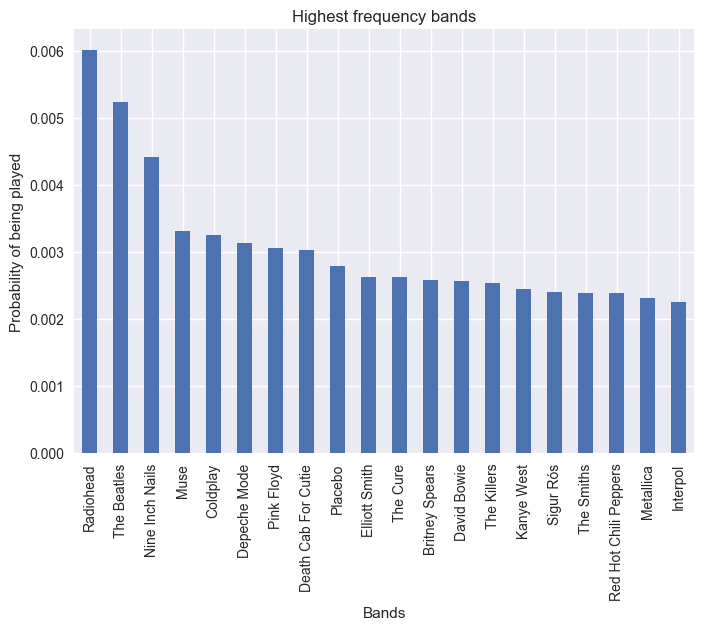
\includegraphics[width=0.9\textwidth]{images/highest_freq_bands.png}
		\caption{Highest frequency bands}
	\end{figure}
	\newline
	So we see the band that is most listened to is Radiohead with a support of 0.6\% of all songs heard. 
	\newline
	\newline
	Then we plot how many bands each user listents to (for 1/3 of the users or 333 users, to accelerate analysis):
	\begin{figure}[ht!]
		\centering
		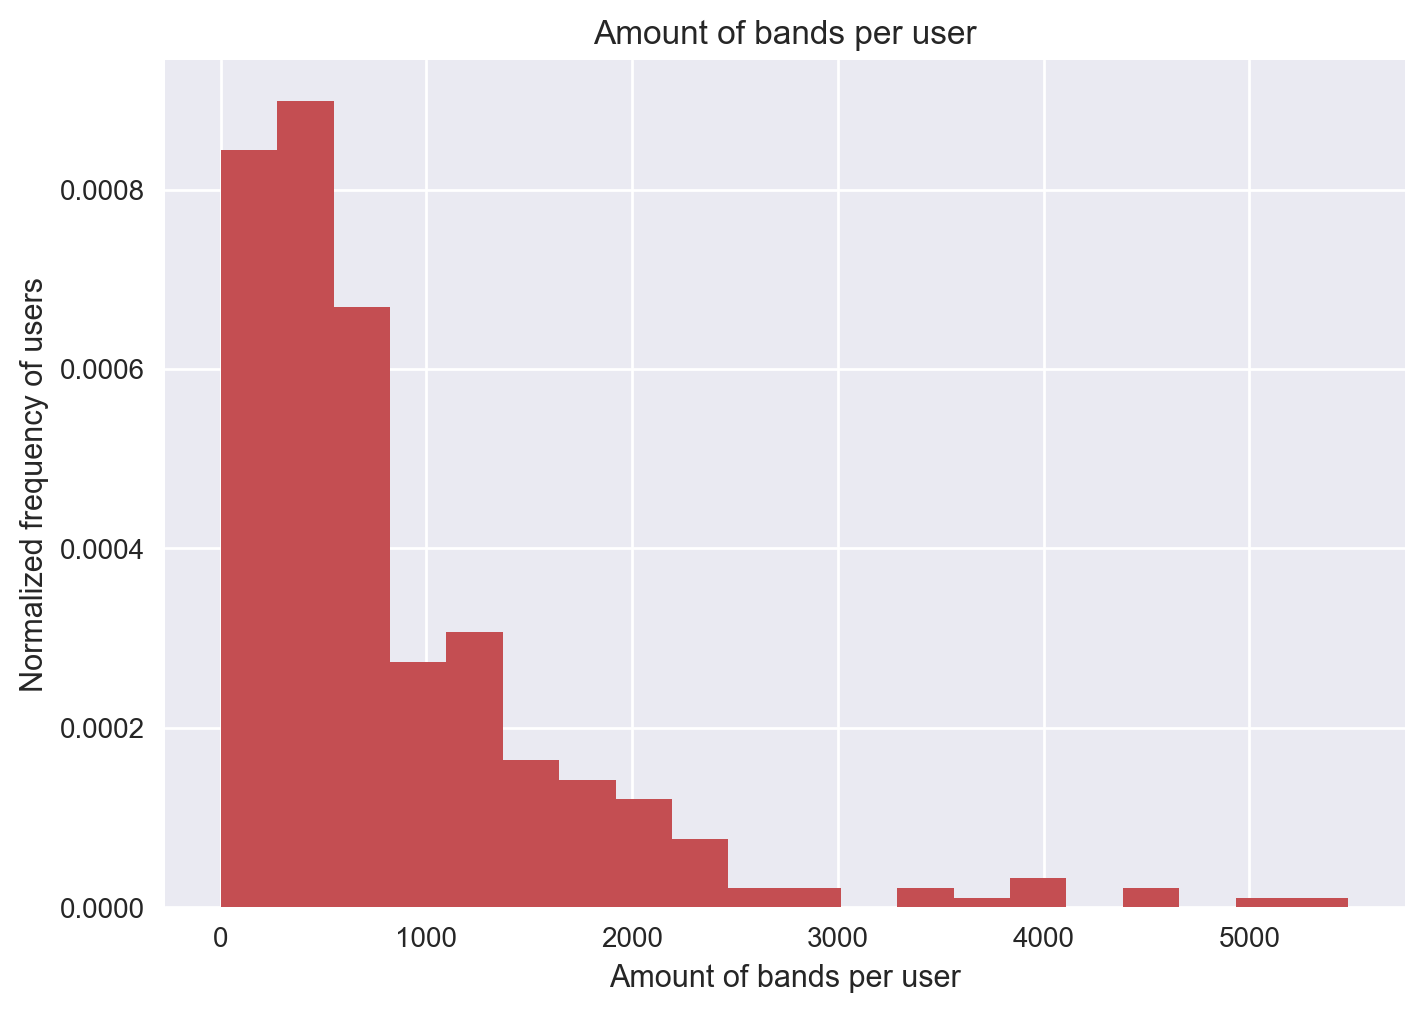
\includegraphics[width=0.9\textwidth]{images/bands_per_user.png}
		\caption{Amount of bands per user (n = 333 users)}
	\end{figure}
	\newline
	Here we see that most listeners listened to anywhere from 2 to 1000 unique bands. The range of bands per user is 2 to 5481 with mean=852.2 and SD=853.7.
	\newline
	\newline
	For the following analyses, we took subsamples of all rows for faster processing, which will be detailed in each part.  
	
	
	
	\subsection{Beethoven recommendations}
	\par\noindent After loading the data as described in \ref{sec:21}, we got a list of all the users that had listened to at least one Beethoven song. Then, from the cleaned data set we kept only those rows with users that listened to something by Beethoven. 
	% \todo{The first two sentences of this paragraph seem to same the same or wasn't able to understand the difference.}
	After sampling the first 500000 rows, we got all the bands with a support of at least 0.7 (Beethoven having a support of 1 or almost 1 because of the sampling).
	\begin{lstlisting}
	items                  support   count
	[1]  {Ludwig Van Beethoven} 0.9629630 26   
	[2]  {Royksopp}             0.8518519 23   
	[3]  {The Killers}          0.8148148 22   
	[4]  {Coldplay}             0.8148148 22   
	[5]  {Depeche Mode}         0.8148148 22   
	[6]  {Bjork}                0.7777778 21   
	[7]  {Air}                  0.7777778 21   
	[8]  {Moby}                 0.7407407 20   
	[9]  {David Bowie}          0.7407407 20   
	[10] {Placebo}              0.7407407 20   
	[11] {Muse}                 0.7407407 20   
	[12] {Pink Floyd}           0.7407407 20   
	[13] {Beck}                 0.7037037 19   
	[14] {Daft Punk}            0.7037037 19   
	[15] {Gorillaz}             0.7037037 19  
	\end{lstlisting}
	\par\noindent While all these bands have a chance of at least 70\% to have been listened by someone who also listened to Beethoven, some of them (e.g., Coldplay, The Killers) are popular in general. For this reason we then analyzed the most popular bands in general, with a support of at least 0.6 and got the following results:
	\begin{lstlisting}
	items               support   count
	[1]  {Coldplay}          0.8181818 18   
	[2]  {Placebo}           0.7272727 16   
	[3]  {The Killers}       0.7272727 16   
	[4]  {David Bowie}       0.7272727 16   
	[5]  {The White Stripes} 0.6818182 15   
	[6]  {Gorillaz}          0.6818182 15   
	[7]  {Radiohead}         0.6818182 15   
	[8]  {Nine Inch Nails}   0.6818182 15   
	[9]  {Air}               0.6363636 14   
	[10] {The Cure}          0.6363636 14   
	[11] {Beck}              0.6363636 14   
	[12] {Arcade Fire}       0.6363636 14   
	[13] {Muse}              0.6363636 14   
	\end{lstlisting}
	
	\par\noindent Based on these 2 lists, a good recommendation would be \textbf{Royksopp}, because this band is not among the popular ones.
	
	\subsection{From Beethoven to Eminem}
	In order to complete this part we loaded the Last.fm dataset, then trimmed the dataset to the two columns as explained before, and finally took a sample of 20\% of the entire dataset. The 20\% of the data is took randomly thanks to the function sample() of R, so it might be that the result is slightly different if loaded more than one time, but the results should be consistent.
	
	After the sampling and the transaction creation for each userid, we generated the frequent itemsets without specifying the maxlen parameter(so that algorithm stops automatically).From this set we kept each item that contained either Beethoven or Eminem in order to focus on the itemsets of our interest. 
	Then it was easy to generate rules from here and use arulesViz in order to create a graph and see path from Beethoven to Eminem.
	There are many paths in the file attached as beethoven\_to\_eminem\.pdf, one of them is for example:\\
	Ludwig Van Beethoven $\rightarrow$ Massive Attack $\rightarrow$ Nelly Furtado $\rightarrow$ Eminem
	
	
	\subsection{Using info about users}
	For this exercise we added the demographic information (sex, age, and country) to the user+band dataset. We randomly sampled 10\% of rows for faster processing.\\
	We made three examples in order to show how a data scientist can discover starting from these three new data.\\
	Each example is divided in a different script:
	
	\begin{itemize}
		\item Ex1, which are the favorites band for Germans(country)? script24\_germans\_favorites.R
		\item Ex2, which are the favorites artists for male(gender) teenagers(age) (categorized between from 14 to 20) from all over the world? script24\_male\_teenagers\_favorites.R
		\item Ex3, which are the favorites musicians for English male teenagers (country,gender,age)? script24\_english\_male\_teenagers\_favorites.R
	\end{itemize}
	
	\subsection{Giving Iron Maiden CD to friend who would actually like it}
	\par\noindent The idea we used in this exercise was to get all the rules where the consequent is Iron Maiden, and sort them by lift. Then, we would choose the top 5 results to add in our questionnaire.
	\par\noindent After implementing this idea we got the following results:
	\begin{lstlisting}
	lhs              rhs    support confidence     lift count
	[1] {Bruce Dickinson} => {Iron Maiden} 0.02391304  0.8800000 9.200000    22
	[2]     {Primal Fear} => {Iron Maiden} 0.01195652  0.7857143 8.214286    11
	[3]      {Hammerfall} => {Iron Maiden} 0.02391304  0.7586207 7.931034    22
	[4]    {Running Wild} => {Iron Maiden} 0.01304348  0.7500000 7.840909    12
	[5]      {Symphony X} => {Iron Maiden} 0.01630435  0.7500000 7.840909    15
	[6]        {W.A.S.P.} => {Iron Maiden} 0.02173913  0.7407407 7.744108    20
	\end{lstlisting}
	
	
	\section{(Bonus) Visualization of Association Rules (10P)}
	
	In this last exercise we used the package "arulesViz" in order to easily plot rules as a graph. In this graph, nodes are our items and edges represent rules. Since it is hard to visualize too many rules at once, we plotted few rules sorted by lift and confidence, since a graph of 10000 nodes is hard to interpret. 
	
	\pagebreak
	\begin{center}
		\begin{figure}[!ht]
			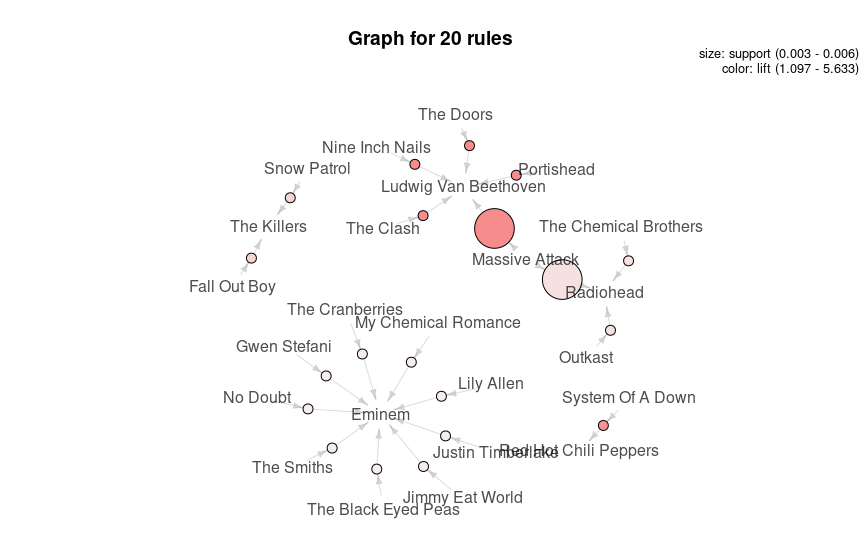
\includegraphics[width=\textwidth]{images/plot1.png}
			\caption{First 20 rules ordered by lift}
		\end{figure}
	\end{center}
	
	\begin{center}
		\begin{figure}[!ht]
			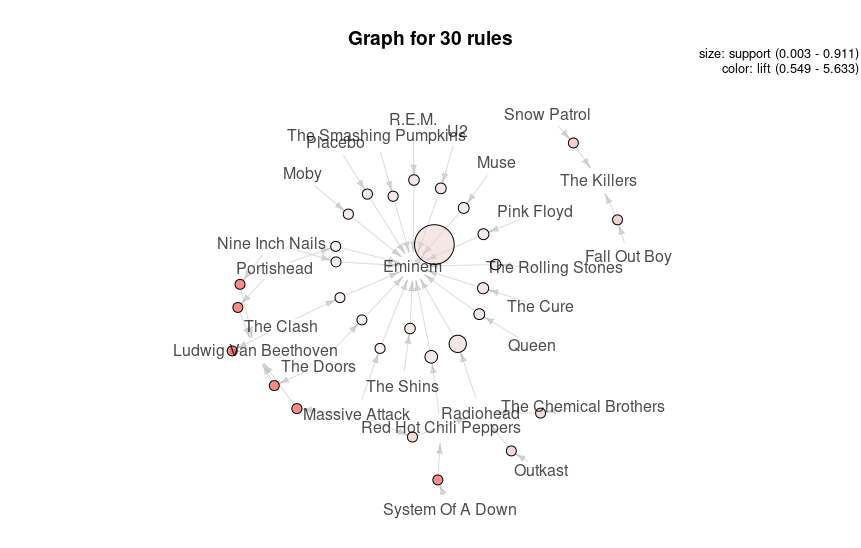
\includegraphics[width=\textwidth]{images/plot2.png}
			\caption{Last 30 rules ordered by confidence}
		\end{figure}
	\end{center}
	
	
	
	\begin{center}
		\begin{figure}[!ht]
			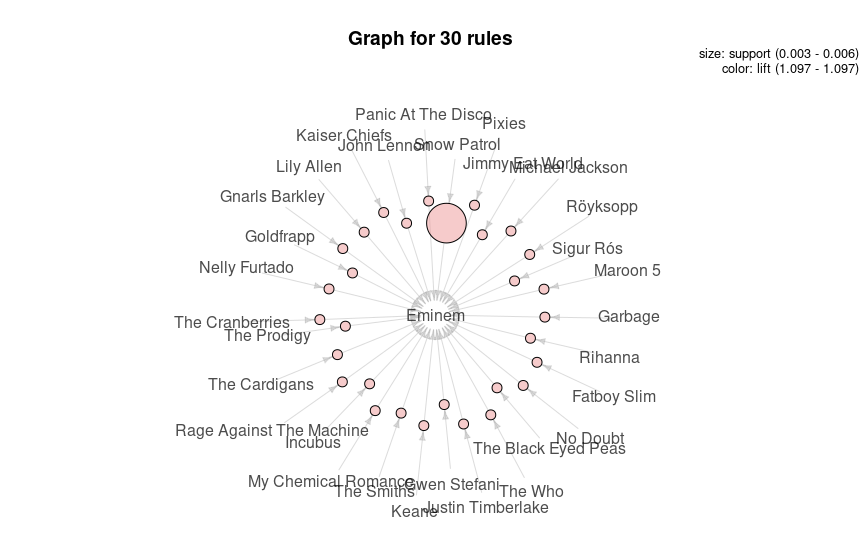
\includegraphics[width=\textwidth]{images/plot3.png}
			\caption{First 30 rules ordered by confidence}
		\end{figure}
	\end{center}
	
	\break Using visualizations with rules, we can see paths from node to node. As in exercise 2.3 (Beethoven to Eminem) this can help us see how we can gradually suggest new artists.\\
	So if we wish to focus on a subset of nodes, we can extract them from our "big" set of rules and plot the ones we are interested in, which is really helpful for data scientists that have to mine data and find new association rules, especially for items that seem to be really "far away" from each other.
	
	% citation section
	
\end{document}

% This is how you write code into Latex:
% \lstinputlisting[language=R,label=lst:r_code,caption=Boxplot example]{code/boxplot.R}